%!TEX root = ../documentation.tex

%% SECTION
\section{Zusammenarbeit während der Implementierung}
\label{sec:implementierung}

Nach der Betrachtung der Zusammenarbeit in verschiedenen Vorgehensmodellen soll vertieft auf die gemeinsame Arbeit während der Implementierung eingegangen werden. Die Implementierung ist hier die Phase, in der auf Grundlage des Designs die nutzbare Software entsteht. Diese Phase kann streng zwischen der Designphase und der Testphase liegen, oder wie in agilen Vorgehensmodellen iterativ eingebettet sein. Unabhängig davon können im wesentlichen drei Bereiche der Zusammenarbeit genannt werden. Als erstes ist das die Übergabe von der Designphase zur Implementierung. Hauptsächlich ist dann die gemeinsame Arbeit an einer Code-Basis während der Implementierung betroffen und abschließend muss eine Übergabe an die Qualitätssicherung erfolgen.
%\\ \todo[tickmarkheight=0.1cm, color=yellow]{Infos zu dem 1. und 3. ausarbeiten}%
Die Ausgestaltung der gemeinsamen Arbeit am Quellcode wird näher betrachtet. Dabei geht es darum Strategien kennenzulernen und den Einsatz von Werkzeugen zu bewerten.
\\
Während der Bearbeitung von Quellcode treten zwei Herausforderungen auf. Zum einen besteht der Wunsch auf ältere Versionen zurückfallen zu können, falls ein Experiment nicht funktioniert. Zum anderen soll es möglich sein, dass mehrere Entwicklerinnen und Entwickler parallel an der gleichen Datei arbeiten können. Naive Lösungen für diese Probleme sind leicht verständlich aber aufwändig. Vor einem Experiment wird eine Sicherheitskopie angelegt. Falls das Experiment scheitert, wird die aktuelle Datei verworfen und wieder durch die Sicherheitskopie ersetzt. Für die gleichzeitige Arbeit an Dateien kann eine Kennzeichnung der Änderungen im Code erfolgen, anschließend ein Austausch der Dateien. Eine der Entwicklerinnen oder einer der Entwickler hat nun die Aufgabe, die Dateien zu vergleichen und die Änderungen in einer resultierenden Datei zusammenzufassen. 
\\
Dass dieses Vorgehen zwar funktioniert, aber nicht sehr effizient ist, ist offensichtlich. Um diese Arbeitsschritte zu automatisieren haben sich Systeme für die Quellcode-Verwaltung entwickelt, die beide Herausforderungen erleichtern. Im Folgenden wird ein kurzer Überblick über diese Systeme gegeben bevor Strategien für die Zusammenarbeit damit vorgestellt werden.


%% SUBSECTION
\subsection{Quellcode-Verwaltungs-Systeme}
\label{sec:implementierung:scm}

Die Entwicklung von Software für die Quellcode-Verwaltung findet bereits seit den Siebziger Jahren statt und hatte mit \emph{IEUPDAT} von IBM \cite{Museum:2022:The-IEBUPDAT:75, IBM:2022:Quick:56} ein erstes rudimentäres Werkzeug. Weitere Systeme waren das \emph{Source Code Control System (SCCS)} \cite{McMillan:2021:A-History:58} oder das \emph{Revision Control System (RCS)} \cite{GNU:2022:GNU-RCS:22} und mit \emph{Concurrent Versions System (CVS)} auch ein System, bei dem mehrere Entwicklerinnen und Entwickler gleichzeitig an einer Datei arbeiten können \cite{McMillan:2021:A-History:58}. Aktuellere Systeme sind z. B. \emph{Git} \cite{Chacon:2022:git---local-branching-on-the-cheap:32}, \emph{Subversion} \cite{The-Apache-Software-Foundation:2022:Apache:94}, \emph{Mercurial} \cite{Mercurial-Community:2022:Mercurial:74} oder \emph{Team Foundation Version Control (TFVC)} \cite{Microsoft:2022:What:67}.
Diese Systeme können nach ihrer grundlegenden Funktionsweise unterschieden werden:
\begin{itemize}
\item
Lokale Versionskontrolle: Lokale Versionierung, oft von einer einzelnen Datei. Z. B. SCCS, RCS
\item
Zentrale Versionskontrolle: Hier ist auch die Kommunikation über das Netzwerk möglich. Wichtig ist, dass der aktuelle Stand des Quellcodes immer auf dem zentralen Server ist. Bei der Bestätigung einer Änderung wird diese auf das zentrale Repository übertragen. Z. B. CVS, Subversion, TFVC
\item
Verteilte Versionskontrolle: Auch hier ist die Netzwerkkommunikation möglich. Oft existiert auch hier ein zentrales Repository, dieses dient aber nur dem gemeinsamen Austausch. Jede Entwicklerin und jeder Entwickler hat ein voll funktionsfähiges lokales Repository.  Z. B. Git, Mercurial
\end{itemize}

Die Plattform \emph{Openhub} \cite{Inc.:2022:Compare:44} veröffentlicht die Verteilung auf Quellcode-Verwaltungs-Systeme von bei ihr gehosteten Projekten.
Im November 2022 hatte Git einen Anteil von 73 Prozent, gefolgt von Subversion mit 22 Prozent sowie Mercurial und CVS mit jeweils einem Prozent. Andere Systeme sind hier nicht relevant. Anzumerken ist, dass hier ausschließlich Open-Source-Projekte in die Statistik fallen, weshalb davon auszugehen ist, dass auch weitere Systeme im Unternehmenskontext relevant sind. Deutlich sichtbar ist aber die Bedeutung von \emph{Git}, weshalb sich diese Arbeit in der Folge auf dieses System konzentriert.


%% SUBSECTION
\subsection{Quellcode-Hosting-Lösungen}
\label{sec:implementierung:hosting}
Es existieren verschiedene Plattformen, die die gemeinsame Bearbeitung von Quellcode und das Hosting von Projekten ermöglichen. Plattformen, die auf Git aufbauen sind z. B. \emph{Github}, \emph{BitBucket} (das ursprünglich rein auf \emph{Mercurial} fokussiert war) und \emph{Gitlab}. Im Gegensatz zur reinen Versionsverwaltung, auf der diese Plattformen aufbauen steht die Zusammenarbeit und das Präsentieren des Projekts im Vordergrund.


%% SUBSECTION
\subsection{Strategien zur Quellcode-Verwaltung}
\label{sec:implementierung:workflows}

Die genannten Quellcode-Verwaltungs-Systeme helfen bei der gemeinsamen Bearbeitung des Quellcodes, die als stetes Aufspalten und Zusammenführen von Quellcode gesehen werden kann. Im Folgenden werden verschiedene Strategien und Workflows vorgestellt, um diesen Vorgang zu gestalten. Diese Strategien lassen sich grundlegend auch mit anderen Quellcode-Verwaltungs-Systemen anwenden, für die Beispiele wird jedoch Git verwendet. Es wird herausgestellt, welche Vor- und Nachteile die Systeme haben und welche Herausforderungen sie haben.
Einige Begriffe sollten eingeführt werden, um Unschärfen zu vermeiden. Das sind die folgenden:
\begin{itemize}
\item
Repository: Der Ort, in den Regel ein Verzeichnis, an dem die Quellcode-Dateien sowie Metadaten und Informationen für die Quellcode-Verwaltung gespeichert sind. Oft gibt es ein \emph{zentrales Repository}, das über das Netzwerk erreichbar ist und zum Austausch im Team dient.
\item
Klonen: Beim Klonen eines, meist zentralen, Repositorys wird eine lokale Kopie erstellt, auf der gearbeitet werden kann. Die Bearbeitungen können später wieder mit dem zentralen Repository vereinigt werden.
\item
Commit: Die \emph{Bestätigung}, dass die Arbeit an Quellcode-Dateien gesichert werden soll. Mit einem Commit wird der aktuelle Stand in die Quellcode-Verwaltung aufgenommen und kann später wieder abgerufen werden oder an ein \emph{zentrales Repository} geschickt werden.
\item
Branch: Eine Folge von \emph{Commits}. Für einen Branch sind mehrere Betrachtungsweisen möglich. Als Beispiel ist ein zentrales Repository gegeben, welches genau einen Branch enthält. Beim Klonen des Repositorys exisitert dieser Branch dann zwei mal. Bei einem Commit auf dem lokalen Branch ändert sich der Branch auf dem zentralen Repository erstmal nicht. Dadurch ergeben sich zwei unterschiedliche Branches, die jedoch den gleichen Namen besitzen können, wobei sich der Speicherort unterscheidet. Das wäre eine Betrachtung von Branches. Im Fall von Git wird auch das dedizierte Erstellen von Branches angeboten, die neben dem \emph{Hauptbranch} existieren und beim Klonen mit berücksichtigt werden. Diese können sowohl im zentralen als auch im lokalen Repository angelegt werden. Das wäre die zweite Betrachtung von Branches.
\item
Mergen:
Wenn mehrere Branches existieren besteht in der Regel die Anforderung, diese zu einem späteren Zeitpunkt wieder zu vereinigen. Dieser Vorgang wird als Mergen bezeichnet. Es bedeutet, dass die Commits aus einem Branch in einen anderen Branch übernommen werden. Dabei kann es zu Konflikten kommen, wenn eine Datei in beiden Branches bearbeitet wurde.
\item
Integration: Das Mergen von Änderungen in den \emph{Hauptbranch} des zentralen Repositorys.
\end{itemize}

Die Betrachtung der folgenden Strategien beruht auf der Annahme, dass jede Version der Software auf der vorangegangenen basiert. Das bedeutet nicht, dass nicht mehrere Versionen gleichzeitig unterstützt und sogar noch mit Hotfixes versehen werden können. Aber wenn an einer Software kundenspezifische Anpassungen vorgenommen wurden, dann dürfen die jeweiligen Anpassungen nur in den Versionen des jeweiligen Kunden oder der Kundin auftauchen. In diesem Fall ist eine komplexere Strategie und mehrere parallele Entwicklungszweige meist notwendig.
\\
Wie Fowler \cite{Fowler:2020:Patterns:07} schreibt, ist nicht das Branchen ein Problem, sondern das spätere Mergen. Deshalb soll zuerst auf die Probleme hierbei eingegangen werden, bevor Strategien zum Branchen vorgestellt werden.

%\todo{wieder einkommentieren}
%Dabei soll einerseits ein vom konreten Workflow unabhäniges Muster gezeigt werden, aber auch konkrete häufig genutzte Workflows. Wichtige Punkte, die beachtet werden sollten sind: 
%\begin{itemize}
%\item
%Integrationshäufigkeit
%\item
%Branch-Pattern
%\item
%Versionierungs-Policy /Art der Software
%\item
%Branches während Entwicklung
%\item
%Branches für den Deploy
%\end{itemize}
%
%Fowler spricht dabei von "Feature Branching vs Continuous Integration". hier sollte beachtet werden, dass sich beides nicht ausschließt.

%% SUBSUBSECTION
\subsubsection{Merging}

%In den vorangegangenen Kapiteln wurden verschiedene Strategien zur gemeinsamen Quellcode-Verwaltung vorgestellt. Dabei lag der Fokus auf dem Branching. Letztlich ist es aber immer ein Aufteilen und wieder zusammenführen, das immer wieder vorkommt. Das zusammenführen, Mergen genannt, ist dabei meist der schwierigere Teil.
Im optimalen Fall ist das Design einer Software so modular und leicht erweiterbar, dass eine Quellcode-Datei nie von mehreren gleichzeitig bearbeitet wird. Dann würde es beim Mergen keine Probleme geben. In der Realität ist es aber oft der Fall, bzw. teilweise notwendig, dass eine Datei parallel bearbeitet wird. In diesem Fall ist eine gute Strategie für das Mergen notwendig, um die auftretenden Konflikte zu minimieren bzw. eine Auflösung zu erleichtern. 
\\
Im Falle, dass es parallele Bearbeitungen einer Datei gibt, lassen sich im wesentlichen zwei Konflikttypen unterscheiden, \emph{textuelle} und \emph{semantische} Konflikte \cite{Fowler:2020:Patterns:07}. Ein textueller Konflikt tritt dabei auf, wenn z. B. der Name einer Klasse von zwei Entwicklerinnen oder Entwicklern jeweils unterschiedlich geändert wird. Ein semantischer Konflikt tritt auf, wenn Entwicklerin A den Name der Klasse ändert, Entwickler B parallel diese Klasse mit ihrem alten Namen verwendet. Während ein textueller Konflikt vom Quellcode-Verwaltungs-System leicht erkannt wird und von den Entwicklerinnen und Entwicklern gelöst werden kann, wird ein semantischer Konflikt nicht erkannt und fällt erst zur Kompilierzeit oder im schlimmsten Fall zur Laufzeit auf. Neben dem technischen Mergen des Quellcodes sind also auch hier eine Strategie und Werkzeuge nötig, um semantische Konflikte zu erkennen, bevor eine Integration stattfindet. 
Eine Möglichkeit sind z. B. \emph{Unit Tests}, die nach dem Mergen der Änderungen auf dem lokalen Repository durchgeführt werden bevor zum zentralen Repository integriert wird. Dadurch wird dafür gesorgt, dass alle Branches auf dem zentralen Repository immer in einem stabilen Zustand sind.
\\
Weitere Herausforderungen ergeben sich aus der Häufigkeit des Mergens, bzw. des Integrierens. Abbildung \ref{fig:branchDiagram} zeigt zwei unterschiedliche Möglichkeiten der Visualisierung von Branches. Dabei wird veranschaulicht, dass mit fortschreitender Zeit Branches immer weiter divergieren, anstatt parallel nebeneinander zu laufen. 
Durch häufiges Integrieren, z. B. mithilfe der Continuous Integration, lässt sich diese Divergenz begrenzen, wodurch das Mergen weniger Konfliktpotential besitzt. Nicht in allen Teams ist das allerdings möglich, da hierfür eine gute Testumgebung notwendig ist \cite{Fowler:2020:Patterns:07}, insbesondere die Open-Source-Community unterscheidet sich hier deutlich vom Unternehmenskontext. 


\begin{figure}
\centering
    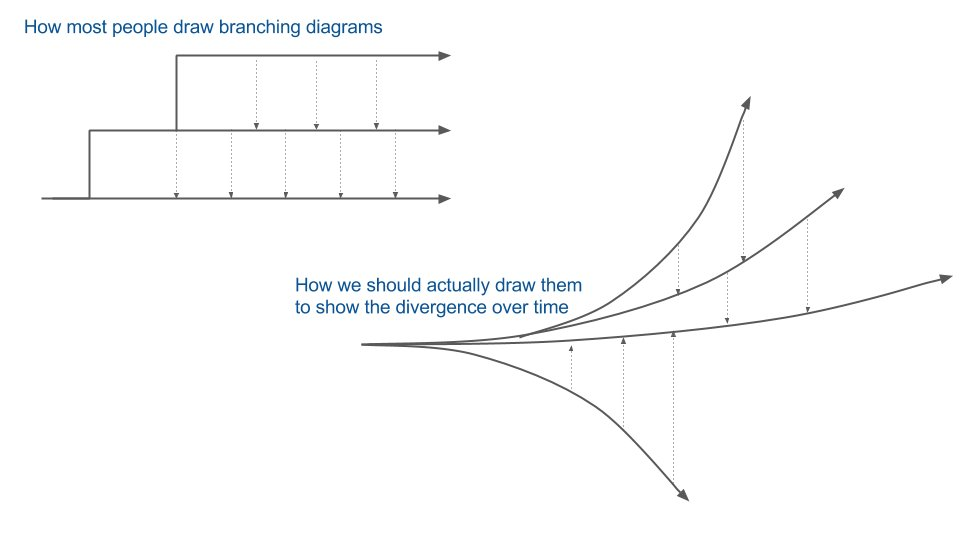
\includegraphics[width=0.7\textwidth, height=0.7\textheight,keepaspectratio]{BranchingDiagram} 
    \caption{Möglichkeiten für die Visualisierung von Branching-Diagrammen. Übernommen von \cite{LeRoy:2017:Twitter:38}}
    \label{fig:branchDiagram}
\end{figure}


%% SUBSUBSECTION
\subsubsection{Ein-Branch-Strategie}
\label{sec:implementierung:workflows:basic}

Der einfachste Workflow besteht darin, dass nur ein Branch genutzt wird. In Git wird dieser inzwischen standardmäßig \emph{main} genannt. Wenn Entwicklerinnen oder Entwickler an einem Feature arbeiten möchten, klonen sie das zentrale Repository und arbeiten auf ihrem lokalen Repository auf dem \emph{main}-Branch. Hier ist also die erste, oben genannte Betrachtungsweise, eines Branches relevant. Wenn das Feature fertig ist, können die Änderungen zurück zum zentralen Repository gepusht werden. Falls dort bereits andere Änderungen committed wurden, muss zuvor ein Merge durchgeführt werden.
\\
Dieser Workflow ist lediglich für wenig komplexe Projekte geeignet, wie z. B. die Erstellung dieser Arbeit, bei der wenige Entwickler beteiligt sind. Ein Nachteil ist, dass ein Commit, der an das zentrale Repository gepusht wird, potentiell für einen instabilen Zustand sorgt. Insbesondere, wenn an einem Feature gearbeitet wird, das länger dauert und aus mehreren Commits besteht, kann es notwendig sein, dass ein Austausch über die bisherigen Commits stattfindet. Der einzige Weg, der hier möglich ist, ist der main-Branch auf dem zentralen Repository. Wenn das unfertige Feature nicht sauber vom Bestandscode getrennt ist, kann es zu Problemen kommen. Der Vorteil ist, dass der Workflow sehr leicht zu verstehen ist. Bei Git wird diese Strategie zum Teil auch als \emph{Basic Workflow} bezeichnet \cite{Antony:2021:5-Different:04}. Die genannten Probleme könnten vermieden werden, wenn dieser Workflow in Kombination mit einer Forking-Strategie (siehe auch Abschnitt \ref{sec:implementierung:workflows:additionalstrategies}) genutzt wird.
\\
Alternativ ist ein Vorgehen nach dem Continuous Integration möglich. Zentraler Punkt hierfür ist das Integrieren sobald ein stabiler Zustand erreicht ist. Dabei muss auch bei länger dauernden Features gewährleistet werden, dass diese abgekoppelt sind, indem z. B. das Interface als letztes implementiert wird \cite{Fowler:2020:Patterns:07} und tatsächlich stabile Zustände erreicht werden. Es findet hier also eine Verlagerung der Arbeit statt. Anstelle aufwändige und fehleranfällige große Merge-Vorgänge durchzuführen, wird der Fokus darauf gelegt, mehr Aufwand in die Erreichung von stabilen Zuständen zu stecken und dafür kleinere, einfachere Merge-Vorgänge zu haben.

%% SUBSUBSECTION
\subsubsection{Multi-Branch-Strategie}
\label{sec:implementierung:workflows:feature}

Eine weitere Möglichkeit, um die Nachteile der Ein-Branch-Strategie zu vermeiden, ist die Nutzung von weiteren Branches neben dem Hauptbranch. 
Durch die Nutzung von eigenen Branches, im Sinne der zweiten, oben genannten Betrachtungsweise, für die Entwicklung von Features, wird der \emph{main}-Branch in einem stabilen Zustand gehalten und trotzdem können auf dem Feature-Branch Commits vorgenommen und auch ausgetauscht werden. 
\\
Die Kernidee besteht darin, dass einzelne Features getrennt voneinander entwickelt werden, und zwar bis sie komplett fertig sind. Da die Feature-Branches aber auch auf dem zentralen Repository gespeichert werden können, ist trotzdem ein Austausch der Änderungen mit anderen Entwicklerinnen und Entwicklern möglich ohne den \emph{main}-Branch in einen instabilen Zustand zu bringen.
Nicht zu unterschätzen ist trotzdem das Problem, die einzelnen Branches wieder in den \emph{main}-Branch zu mergen. Denn auch wenn die einzelnen Features inhaltlich unabhängig sind, kann es vorkommen, dass an den gleichen Stellen Änderungen im Bestandscode notwendig sind.
\\
Ein konkretes Beispiel für diese auch \emph{Feature-Branching} gennannte Strategie ist \emph{git-flow} \cite{Driessen:2010:A-successful:47}. Folgende Branches existieren in diesem Workflow:
\begin{itemize}
\item
Main (oder Master): Dieser spiegelt zu jeder Zeit einen Stand wider, der ausgeliefert werden kann. Zusammen mit Develop bilden sie die Haupt-Branches.
\item
Develop: Dieser spiegelt den aktuellen Stand der Entwicklung wider. Von diesem Branch gehen Feature- und Release-Branches ab und hierhin wird integriert.
\item
Feature Branches: Werden von Develop abgespalten und dorthin integriert. Sind für die dedizierte Entwicklung von Features vorgesehen.
\item
Release Branches: Werden von Develop abgespalten, um unabhängig von weiteren Integrationen nach Develop letzte Fehler zu korrigieren und einen stabilen Zustand herzustellen, der nach Main integriert werden kann. Wird auch wieder zurück nach Develop integriert.
\item
Hotfix Branches: Werden von Main abgespalten, um einen schlimmen Fehler einer veröffentlichten Version zu beheben. Wird wieder nach Main und Develop integriert.
\end{itemize}

%%% SUBSUBSECTION
%\subsubsection{Git Flow}
%\label{sec:implementierung:workflows:gitflow}

%%% SUBSUBSECTION
%\subsubsection{OneFlow}
%
%Als Alternative zu \emph{Git Flow} wird \emph{OneFlow} von Adam Ruka als leichtere Alternative vorgeschlagen. Kernidee ist, dass es genau einen Branch gibt, der dauerhaft ist. Die Entwicklung wird auf kurzlebigen Feature-Branches gemacht. 


%%% SUBSUBSECTION
%\subsubsection{Gitlab Flow}
%\label{sec:implementierung:workflows:gitlabflow}





%% SUBSUBSECTION
\subsubsection{Weitere Strategien}
\label{sec:implementierung:workflows:additionalstrategies}

Neben den ausführlich beschriebenen Strategien, die zu den am häufigsten beschriebenen gehören, gibt es weitere, die je nach Anwendungsumfeld eine Alternative darstellen können. Dabei entstehen beständig neue Vorschläge oder Varianten, um sich an die neuen Entwicklungsumgebungen und Anforderungen anzupassen. Dazu gehören z. B. der \emph{Forking Workflow} \cite{Antony:2021:5-Different:04}, \emph{OneFlow-Workflow} \cite{Ruka:2017:OneFlow:24} oder \emph{Github Flow} \cite{Chacon:2011:GitHub:63}.
\\
Der \emph{Forking-Workflow} hat sich insbesondere in der Open-Source-Community und mit der Verbreitung von Plattformen wie GitHub oder GitLab durchgesetzt, wo zum Teil viele Entwicklerinnen und Entwickler mit unterschiedlichen Arbeitsweisen zusammenarbeiten. Anstelle eines einzigen zentralen Repositorys, zu dem alle ihre Änderungen pushen besitzt jeder ein eigenes zentrales Repository (ein sogenannter \emph{Fork}) auf dem gearbeitet wird. Dadurch können lokale Änderungen veröffentlicht und geteilt werden, um beispielsweise Feedback zu erhalten, ohne das originale Repository in einen instabilen Zustand zu bringen. Der Vorteil besteht darin, dass die Besitzerin oder der Besitzer des originalen Repositorys keinen weitreichenden Zugriff auf das Repository an viele Entwicklerinnen und Entwickler gewähren muss. Über Pull-Requests kann jedoch eine Anfrage an das originale Repository gestellt werden, die Änderungen auch dort zu integrieren. Dieser Workflow kann je zentralem Repository mit anderen Workflows kombiniert werden, sodass an einem Fork auch mehrere arbeiten können.
\\
\emph{OneFlow} ist ebenso wie \emph{Github Flow} eine Reaktion auf den \emph{GitFlow-Workflow}, der für moderne Web-Entwicklung nicht mehr optimal war und als zu komplex und fehleranfällig betrachtet wurde \cite{Ruka:2015:GitFlow:46}\cite{Chacon:2011:GitHub:63}. Die Kernidee ist hierbei, möglichst wenige langlebige Branches zu haben, um die Versionsgeschichte möglichst klar zu lassen. Ein weiterer Vorteil weniger Branches ist, dass es weniger Verwirrung über die richtige Verwendung der Branches und weniger Probleme beim Mergen gibt. Dies wird erreicht, indem sehr häufig integriert wird und der main-Branch immer in einem stabilen Zustand gehalten wird, z. B. mithilfe von selbsttestendem Code. Insbesondere bei der Webentwicklung und Continuous Delivery/Deployment vereinfacht das die Arbeit unter der Voraussetzung.

%% SUBSECTION
\subsection{Grenzen von Git}

Bei der Wahl einer Strategie sollte auch berücksichtigt werden, welche Artefakte während der Implementierung anfallen. Insbesondere Binärdateien können dabei problematisch sein. Binärdateien können zum Beispiel 3D-Modell-Daten sein \cite{Community:2022:Blender:13}. Auch hier fallen oft lediglich kleine Anpassungen an, sodass es unnötig wäre, während des Zusammenführens die komplette Datei zu kopieren. Dies ist aber notwendig, da Git bei Binärdateien nicht nur die Änderungen speichern kann. Dadurch erhöht sich der Speicherbedarf des Repositorys stark und auch die Performance kann darunter leiden, wenn jedes Mal viele Daten übertragen werden müssen. Hier muss eine Einschätzung getroffen werden, wie häufig Binärdateien geändert werden und wie groß diese sind. Wenn nur wenige, kleine Binärdateien im Repository vorhanden sind, die zudem selten geändert werden, zum Beispiel finale Dokumentations-PDFs, kann Git ohne Bedenken genutzt werden. Im Falle vieler, potentiell großer Binärdateien, wie zum Beispiel bei der Entwicklung von 3D-Computerspielen stellt dies einen Einsatz von Git in Frage. Zur Lösung dieses Problems gibt es Ansätze als Erweiterungen von Git \cite{Kenlon:2016:Hot-to-manage:74}. Der Kerngedanke ist dabei, dass nicht die Binärdateien selbst im Repository gespeichert sind, sondern Zeiger auf diese Dateien \cite{Gehman:2019:How-Git-LFS-Works::74}. Dadurch kann der Speicherbedarf und die Performance von Git optimiert werden. Die Versionierung und parallele Bearbeitung der Binärdateien muss dann aber durch das entsprechende Bearbeitungsprogramm sichergestellt werden können.

%% SUBSECTION
\subsection{Zwischenfazit}

Die vorgestellten Strategien bieten eine Grundlage für die Entscheidungsfindung bei der Wahl von Richtlinien und Werkzeugen während der Zusammenarbeit bei der Implementierung. Nicht vergessen werden sollte, dass diese Strategien nicht für sich stehen und auch keinen Anspruch auf Gültigkeit erheben. Sie müssen immer im Kontext der gesamten Entwicklungsumgebung stehen und natürlich gegebenenfalls an die konkrete Situation im Projektteam angepasst werden. In diesem Zusammenhang ist auch eine Abstimmung mit der Strategie des Qualitätsmanagements notwendig, auf das im Folgenden näher eingegangen wird.
Eine Untersuchung zur Softwarequalität in Abhängigkeit der Branching-Strategie kam dabei zu dem Ergebnis, dass zu viele Branches einen negativen Einfluss haben und die Branching-Strategie mit der Software-Architektur und der Team-Struktur abgestimmt sein sollte, um negative Konsequenzen zu vermeiden \cite{Shihab:2012:The-Effect:91}.



